\documentclass[a4paper,12pt]{book}
%\documentclass[a5paper,12pt,landscape]{book}
%\documentclass[a5paper,12pt,landscape]{report}

\usepackage[margin=3cm]{geometry}

\usepackage[T1]{fontenc}
\usepackage[english]{babel}
%\usepackage[utf8]{inputenc}

\usepackage{tikz}
\usetikzlibrary{calc}
\usetikzlibrary{arrows, backgrounds}
\usetikzlibrary{matrix, arrows.meta}
\usetikzlibrary{decorations.pathreplacing}

%\usepackage{amsfonts}
%\usepackage{amsmath}
%\usepackage{amsthm}
\usepackage{bm}

% Used for split environment
\usepackage{amsmath}
% Separate rows in align environment by this amount
\addtolength{\jot}{1em}

\usepackage{graphicx}
\graphicspath{{../fig/} {fig/}}
\usepackage{subfig}
\usepackage{wrapfig}

\usepackage{caption}
\captionsetup{font=footnotesize}

\newcommand*\V[1]{\bm{#1}}
\newcommand{\E}{\V{E}}
\newcommand{\B}{\V{B}}
\renewcommand*{\v}{\V{v}}
\newcommand{\x}{\V{x}}
\newcommand{\dt}{\Delta t}
\newcommand{\dx}{\Delta x}

\title{Simulation of plasma with \texttt{cpic} using OmpSs}
\author{Rodrigo Arias Mallo}
\date{\today}

\begin{document}

\maketitle
\tableofcontents

\chapter{Introduction}
\label{ch:intro}

It may be surprising to find out that the most common state of matter is plasma 
when we look at the universe. A plasma is an ionized gas consisting of ions and
free electrons distributed over a region in space.
in which at least one electron 
of the atom is separated, so it remains positively charged (ionized) 
\cite{chen}.  Usually this happens in the vacuum

\section{Motivation}

% Why?

\section{Objectives}

\section{Context}

\section{Structure}

\begin{wrapfigure}{r}{0.3\textwidth}
\centering
\scalebox{0.7} {
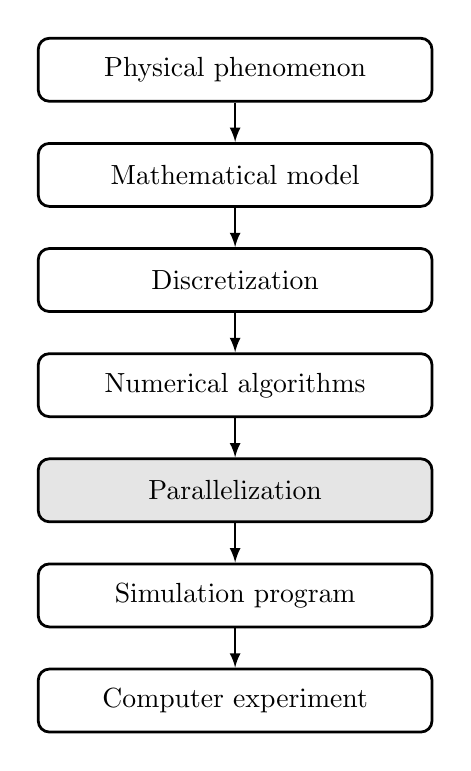
\begin{tikzpicture}[>=latex,thick]
	\matrix (m) [
		matrix of nodes,
		column sep=5mm,
		row sep=5mm,
		nodes={
			draw, % General options for all nodes
			line width=1pt,
			anchor=center,
			text centered,
			rounded corners,
			minimum width=5cm,
			minimum height=8mm,
		},
		txt/.style={text width=1.5cm,anchor=center},
	]
	{
		Physical phenomenon \\
		Mathematical model \\
		Discretization \\
		Numerical algorithms \\
		|[fill=black!10]| Parallelization \\
		Simulation program \\
		Computer experiment \\
	};
	\foreach \i [evaluate={\j=int(\i+1)}] in {1,...,6}{
		\draw[->] (m-\i-1) -- (m-\j-1);
	}

\end{tikzpicture}
}
\caption{Principal steps in computer experiment}
\label{fig:structure}
\end{wrapfigure}

The structure of the document follows the diagram shown in the 
figure~\ref{fig:structure}. In chapter~\ref{ch:intro}, plasma is described as a 
physical phenomenon and we focus on the relevant properties that we want to 
study, from which we derive a mathematical model.  In 
chapter~\ref{ch:plasma-sim} and~\ref{sec:test}. The discretization of the 
mathematical model allows the computer simulation by using numerical algorithms.

\chapter{Related work}

The simulation of plasma began with the first simulations in the 1950s with the
John Dawson codes for 1D simulation. In 1965 Hockney and Buneman introduced the
direct Poisson solver, which allowed the first useful electrostatic simulations.
In the 1970s, the theory of electrostatic PIC was developed by Langdon, leading
to the first electromagnetic codes.

Finally, from 1980 to the 90s the two main bibles of particle-in-cell codes were
produced  by B. Langdon and C. Birdsall in 1975 \cite{birdsall} and by Hockney
and Eastwood in 1988 \cite{hockney}.

At the Plasma Theory and Simulation Group of the University of California,
Berkeley the XOOPIC \cite{xoopic} family of well known codes were released in
the 1990s.

The are a lot of specific PIC codes which are currently used for the simulation
of various phenomena, mostly centered in fusion reactors: ELMFIRE, GENE, GTC,
ORB5, PAR-T and EUTERPE \cite{euterpe}.



\part{Theory\\ \small \textit{No C code here}}

% What is a plasma: write about the physical phenomenon
\chapter{Plasma introduction}
\label{ch:plasma-intro}

% Write about how plasma can be simulated with a computer. The methods regarding 
% *only* on numerical methods to simulate plasma, not the specific to HPC ones.

\section{Everyday plasmas}

It may be surprising to find out that when we look at the universe, the most
common state of matter is plasma, which is a ionized gas formed by free
electrons and ions at a region in space--often known as the fourth state of
matter. The sun, our closest star, is a giant
ball of plasma 


Most common forms of plasma only occur in vaccum, as otherwise the air cools the
plasma and returns to a gas.

In our planet, we can see forms of plasma almost every day. A storm day the
lightnings. The spark on some piezoelectric lighters, which is the very same
principle that occurs in gasoline engines.

The Aurora Borealis, of the lightning of a fluorescent tube or the pixels of a
plasma TV.

A precise definition of a plasma is given by Chen~\cite{chen} as \textit{``a
quasineutral gas of charged and neutral particles which exhibits collective
behavior''}. The 


% Begin the simulation of plasma part
\chapter{Plasma simulation}
\label{ch:plasma-sim}

% Write about how plasma can be simulated with a computer. The methods regarding 
% *only* on numerical methods to simulate plasma, not the specific to HPC ones.

\section{The particle-in-cell method}

%TODO: Show the main equation
Solving the Vaslov equation requires a large amount of numerical resources. The 
particle in cell method, approximates the solution by discretization of the 
fields.

The method is divided in four main phases: 

\begin{itemize}
\item Particle motion.
\item Charge accumulation.
\item Solve field equation.
\item Interpolation of fields in particle position.
\end{itemize}


%\section{1D electrostatic simulation}
%The magnetic field is ignored.
%
%\section{2D simulation}
%The magnetic field is not ignored.
%
%\section{Electromagnetism}
%
%\subsection{Background magnetic field}
%
%To introduce the magnetic field, the equations are:
%
%$$ $$

\section{Particle mover}

In order to move the particles, the equations of motion need to be solved:
%
\begin{equation}
m \frac{d\v}{dt} = q (\E + \v \times \B)
\end{equation}
\begin{equation}
\frac{d\v}{dt}=\v
\end{equation}
%
Several methods are available, but we will focus on the Boris integrator.

\subsection{Boris integrator}

Consists of three steps:
%
\begin{enumerate}
\item Add half of the electric impulse
\item Rotate
\item Add the remaining half electric impulse
\end{enumerate}
%
The Boris integrator computes the velocity of a particle in a constant electric 
field $\E$ and a constant magnetic field $\B$. We have the velocity 
$\v_{t-\Delta t/2}$ of the particle at $t-\Delta t/2$ as we use the leapfrog 
integrator.
%
\begin{figure}[h]
\centering
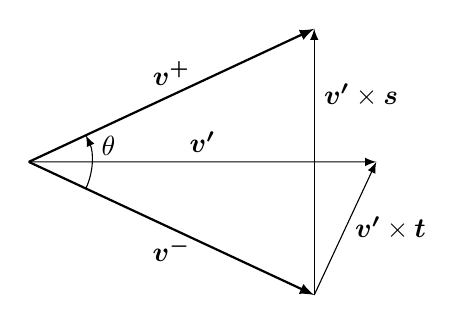
\begin{tikzpicture}[
	scale=2,
	>=latex]

	\def\centerarc[#1](#2)(#3:#4:#5)% Syntax: [draw options] (center) (initial angle:final angle:radius)
		{\draw[#1] ($(#2)+({#5*cos(#3)},{#5*sin(#3)})$) arc (#3:#4:#5); }

	\def\startangle{-25}
	\def\midangle{0}
	\def\endangle{25}
	\def\radius{2.0}
	\pgfmathsetmacro{\vlen}{\radius*tan(\startangle)}%

	\coordinate (O) at (0,0);
	\coordinate (S) at (\startangle:\radius);
	\coordinate (E) at (\endangle:\radius);

%	\centerarc[dashed](O)(\startangle:\endangle:\radius);
	\centerarc[->](O)(\startangle:\endangle:0.2*\radius);

	\draw (O)+(0.4,0.1) node [right] {$\theta$};

	\draw [thick,->] (O) -- (E) node [midway, above] {$\V{v^+}$};
	\draw [thick,->] (O) -- (S) node [midway, below] {$\V{v^-}$};

	\path (S) +(\startangle-90:\vlen) coordinate (V1E);
%	\path (E) +(\endangle-90:\vlen) coordinate (V3E);

%	%\draw [->] (E) -- (V3E);
	\draw [->] (S) -- (V1E) node [midway, right] {$\V{v'} \times \V t$};
%
	\draw [->] (O) -- (V1E) node [midway, above] {$\V{v'}$};
	\draw [->] (S) -- (E) node [near end, right] {$\V{v'} \times \V s$};

%	\draw [fill=white] (O) circle (0.02);

\end{tikzpicture}
\caption{Velocity space rotation from $\v-$ to $\v+$}
\end{figure}
%
\paragraph{Add half electric impulse} We define $\V{v^-}$ as the velocity after 
half a electric impulse:
$$\v^- = \v_{t-\dt/2} + \frac{q \E}{m} \frac{\dt}{2}$$

\paragraph{Rotate for the magnetic field} The rotation is done in two steps, 
first the half rotation is computed, with an angle of $\theta/2$:
$$\v' = \v^- + \v^- \times \V t $$

Then the rotation is completed by symmetry, using the $\V s$ vector
$$ \V s = \frac{2 \V t}{1 + \V t^2} $$
as
$$ \V{v^+} = \V{v^-} + \V{v}' \times \V{s} $$

\section{Charge accumulation}

The charge density $\rho$ is a scalar field

\section{Field equations}

Once we have the charge density $\rho$ we can compute the electric field $\E$ by 
the integration of the field equations
%
\begin{equation}
\E = -\nabla \phi
\end{equation}
\begin{equation}
\nabla \cdot \E = \frac{\rho}{\epsilon_0}
\end{equation}
%
Which can be combined into the Poisson equation
%
\begin{equation}
\label{eq:poisson}
\nabla^2\phi = - \frac{\rho}{\epsilon_0}
\end{equation}
%
Different methods can be used to obtain the electric field, but we will focus on 
matrix and spectral methods.


\chapter{Discrete model}
\label{ch:discrete-model}

\epigraph{... all models are approximations. Essentially, all models are wrong, but some
are useful. However, the approximate nature of the model must always be borne in
mind....}{Empirical Model-Building and Response Surfaces, 1987---George E. P.  
Box}

The mathematical model is discretized in algebraic operations, in order to be 
computable.

\section{Charge assignment}
At each grid point $g$ at $\x$ we accumulate the charge of each particle $p$ in 
$\x_p$ as
%
\begin{equation}%{{{
\rho(\x) = \sum_p q\,W(\x - \x_p) + \rho_0
\label{eq:charge-accumulation}
\end{equation}%}}}
%
The background charge density $\rho_0$ is used to neutralize the total charge 
when is non-zero. The weighting function $W$ determines the shape of the 
particle charge. Different schemes can be used to approximate the charge density 
from the particles. We will focus on bilinear interpolation for it's simplicity 
and low computation requirements. The corresponding weighting function can be 
written as
%
\begin{equation}%{{{
W(\x) =
\begin{cases}
			\displaystyle\left(1 - \frac{|x|}{\Delta x}\right)
				\left(1 - \frac{|y|}{\Delta y}\right) & \text{if}\ -\Delta\x < \x < 
				\Delta \x\\
			0 & \text{otherwise}
\end{cases}
\end{equation}%}}}
%
Notice that a particle $p$ always affects the four enclosing grid points in the 
neighbourhood $\neigh{p}$, but more complex interpolation methods may extend the 
update region even further. It may be noted that the increase in smoothing, at 
computation expense, can gain from the reduced number of particles needed to 
obtain a similar result, avoiding nonphysical effects.
%
\begin{figure}[]%{{{
\centering
\begin{tikzpicture}[
		>=latex,
		effect/.style={dashed,-{Latex[length=3mm, width=1mm]}},
		particle/.style={fill=black,radius=3pt},
	]
	\draw [step=2cm,dotted] (1,1) grid (5,5);
	\coordinate (p) at (2.5,3.2);
	\coordinate (center) at (3,3);
	\coordinate (A) at ($(center)+(-1,1)$);
	\coordinate (B) at ($(center)+(1,1)$);
	\coordinate (C) at ($(center)+(1,-1)$);
	\coordinate (D) at ($(center)+(-1,-1)$);
	\draw[effect] (p) -- (A);
	\draw[effect] (p) -- (B);
	\draw[effect] (p) -- (C);
	\draw[effect] (p) -- (D);
	\node[above left]  at (A) {$A$};
	\node[above right] at (B) {$B$};
	\node[below right] at (C) {$C$};
	\node[below left]  at (D) {$D$};
	\draw[particle] (p) circle;
	\node[left] at (p) {$p$};
\end{tikzpicture}
\hspace{0.5cm}
\begin{tikzpicture}[
		>=latex,
		box/.style={black},
		particle/.style={fill=black,radius=3pt},
		div/.style={dashed},
	]
	\draw [step=2cm,dotted] (1,1) grid (5,5);
	\coordinate (p) at (2.5,3.2);
	\coordinate (center) at (3,3);
	\coordinate (A) at ($(p)+(-1,1)$);
	\coordinate (B) at ($(p)+(1,1)$);
	\coordinate (C) at ($(p)+(1,-1)$);
	\coordinate (D) at ($(p)+(-1,-1)$);
	\draw[box] (A) -- (B) -- (C) -- (D) -- (A);
	\draw[div] ($(A)!(center)!(B)$) -- (center);
	\draw[div] ($(B)!(center)!(C)$) -- (center);
	\draw[div] ($(C)!(center)!(D)$) -- (center);
	\draw[div] ($(D)!(center)!(A)$) -- (center);
	\node at ($(center)!0.5!(A)$) {$a$};
	\node at ($(center)!0.5!(B)$) {$b$};
	\node at ($(center)!0.5!(C)$) {$c$};
	\node at ($(center)!0.5!(D)$) {$d$};
	\draw[particle] (p) circle;
\end{tikzpicture}
\hspace{0.5cm}
\begin{tikzpicture}[
		>=latex,
		box/.style={black},
		particle/.style={fill=black,radius=3pt},
		div/.style={dashed},
	]
	\draw [step=2cm,dotted] (1,1) grid (5,5);
	\coordinate (p) at (2.5,3.2);
	\coordinate (center) at (3,3);
	\coordinate (A) at ($(center)+(-1,1)$);
	\coordinate (B) at ($(center)+(1,1)$);
	\coordinate (C) at ($(center)+(1,-1)$);
	\coordinate (D) at ($(center)+(-1,-1)$);
	\draw[box] (A) -- (B) -- (C) -- (D) -- (A);
	\draw[div] ($(A)!(p)!(B)$) -- (p);
	\draw[div] ($(B)!(p)!(C)$) -- (p);
	\draw[div] ($(C)!(p)!(D)$) -- (p);
	\draw[div] ($(D)!(p)!(A)$) -- (p);
	\node at ($(p)!0.5!(A)$) {$c$};
	\node at ($(p)!0.5!(B)$) {$d$};
	\node at ($(p)!0.5!(C)$) {$a$};
	\node at ($(p)!0.5!(D)$) {$b$};
	\draw[particle] (p) circle;
\end{tikzpicture}
\caption{Interpolation of particle $p$ charge into the four grid points A to D.}
\label{fig:interpolation}
\end{figure}%}}}
%
The particle $p$ has a uniform charge area, centered at the particle position 
$\x_p$, with size $\Delta \x$, as shown in the figure~\ref{fig:interpolation}.  
Each grid point $A,B,C$ and $D$ receives the amount of charge weighed by the 
area $a,b,c$ and $d$. It can be observed that the area is equal to the opposite 
region, when the particle $p$ is used to divide the grid cell.
%
The particle shape can be altered later in the Fourier space, without large 
computation effort, in case the solver already computes the FFT.
%
\section{Field equations}

In order to compute the electric field $\E$, the electric potential $\phi$ is 
generally needed, which can be obtained from the charge density $\rho$.

\subsection{Electric potential}
Several methods are available to solve the Poisson equation 
(Eq.~\ref{eq:poisson}).

\paragraph{Iterative  methods} such as Jacobi, Gauss-Seidel, Successive Over 
Relaxation (SOR), Chebyshev acceleration are some of the most familiar methods 
to solve the Poisson equation.

\paragraph{Matrix methods} The equations from finite differencing the mesh are 
considered a large system of equations. We can find in this methods the Thomas 
Tridiagonal algorithm, Conjugate-Gradient, LU or Incomplete Decomposition.

\paragraph{Spectral methods} Also known as Rapid Elliptic Solvers (RES) are a 
family of methods that use the fast Fourier transform (FFT). Are know for being 
usually faster than the previous ones, with a complexity in $O(N_g \log_2 N_g)$

\vspace{1em}
\noindent
%
We will only focus on the LU for small problems and for testing, and spectral 
methods, more specific on the Multiple Fourier Transform (MTF) method, as it is 
the main method implemented in the simulator, due to its relative simplicity and 
low computational complexity.

\subsection{LU decomposition}
%
% TODO: Check the error bound
For two dimensions, we can approximate the solution using the second order 
centered finite differences (with an error proportional to $\Delta x ^2 \Delta 
y^2$), as
%
\begin{equation}%{{{
\label{eq:discrete-poisson}
\frac{\phi(x-1, y) + \phi(x, y-1) - 4\phi(x,y) + \phi(x+1,y)+\phi(x,y+1)}{\Delta 
x ^2 \Delta y^2} = - \frac{\rho(x,y)}{\epsilon_0}
\end{equation}%}}}
%
which leads to a system of $N_g$ linear equations and can be also written in 
matrix form
%
\begin{equation}
\label{eq:eq-system}
A\phi = -\frac{\Delta x ^2 \Delta y^2\,\rho}{\epsilon_0}
\end{equation}
%
The $N_g \times N_g$ coefficient matrix $A$ has non-zero coefficients only at 
$a_{ii} = 4$ and $a_{ij} = -1$ with $j \in \{i+1, i-1, i+N_x, i-N_x\} \mod N_x$, 
for all $0 \le i \le Ng$.
%
However, the matrix $A$ is singular, so the system of equations has infinite 
solutions. Boundary conditions can be added to get a unique solution. The extra 
equation $\phi(0,0) = 0$ leads to a system with only one solution, but with one 
extra equation. In order to keep the matrix $A$ square, the following steps may 
be taken:

\begin{enumerate}
\item Subtract  the extra equation $\phi(0,0) = 0$ to the first row of $A$, with 
the only change in the coefficient to $a_{11} = 3$.

\item Add all first $N_g$ equations: Each equation has one coefficient of $4$ 
and four of $-1$ except the first equation. Also we assume the total charge 
density is zero, obtaining $\phi(0,0) = 0$.

\item Subtract it from the last equation, which leads to a zero coefficient that 
can be removed.
\end{enumerate}
%
The only change that remains is at the coefficient $a_{11} = 3$. Now the matrix 
$A$ is squared and non-singular and has only one solution and can now be solved 
with the $LU$ method.

The $LU$ decomposition, with a complexity in $O(2/3N_g^3)$, can be used to form 
two systems of equations that can be solved faster. If we rewrite the system of 
equations~\ref{eq:eq-system} as the usual form $Ax=b$ with
\begin{equation}
x = \phi,\quad b = -\frac{\Delta x ^2 \Delta y^2\,\rho}{\epsilon_0}
\end{equation}
%
Then we can use the decomposition $A=LU$ to form two systems of equations
%
\begin{equation}
\label{eq:LU-systems}
Ux=y, \quad Ly=b
\end{equation}
%
which can be solved in complexity $O(2N_g^2)$.


\subsection{Multiple Fourier Transform (MFT)}

The general second-order PDE with constant coefficients and periodic boundary 
conditions
%
\begin{equation}%{{{
\label{eq:gen-fd}
a \frac{\partial^2 \phi}{\partial x^2}+b\frac{\partial \phi}{\partial x}+c\phi +
d \frac{\partial^2 \phi}{\partial y^2}+e\frac{\partial \phi}{\partial y}+f\phi = 
g(x,y)
\end{equation}%}}}
%
can be solved by using the FFT. If we expand $\phi$ and $g$ in a finite double 
Fourier series, we obtain
%
\begin{equation}%{{{
\phi(x,y) = \sum_{k,l} \hat \phi(k, l) \exp\left({\frac{2\pi i (xk + 
yl)}{n}}\right)
\end{equation}%}}}
%
and
%
\begin{equation}%{{{
g(x,y) = \sum_{k,l} \hat g(k, l) \exp\left({\frac{2\pi i (xk + yl)}{n}}\right)
\end{equation}%}}}
%
which now can be substituted in the Eq.~\ref{eq:gen-fd}, to obtain
%
\begin{equation}%{{{
\hat \phi(k,l) = \hat G(k,l) \, \hat g(k,l),\quad 0<k<N_x,\,0<l<N_y
\end{equation}%}}}
%
with for a unit mesh
%
\begin{equation}%{{{
\begin{split}
\hat G(k,l) = \Bigg[
& 2a \left( \cos \frac{2\pi k}{n} - 1 \right) +
ib \sin \frac{2\pi k}{n} + c \,+ \\
& 2d \left( \cos \frac{2\pi l}{n} - 1 \right) +
ie \sin \frac{2\pi l}{n} + f
\Bigg]^{-1}
\end{split}
\end{equation}%}}}
%
To solve the Poisson equation, discretized as Eq.~\ref{eq:discrete-poisson}, we 
have $a=d=1$ and $b=c=e=f=0$ so we can simplify $\hat G(k,l)$ as
%
\begin{equation}%{{{
\hat G(k,l) = \frac{1}{2}\left[
\cos \frac{2\pi k}{n} +
\cos \frac{2\pi l}{n} -
2 \right]^{-1}
\end{equation}%}}}
%
Let $g = -{\Delta x ^2 \Delta y^2\,\rho}/{\epsilon_0}$, then the steps to 
compute the electric potential can be summarized as follows:
%
\begin{center}%{{{
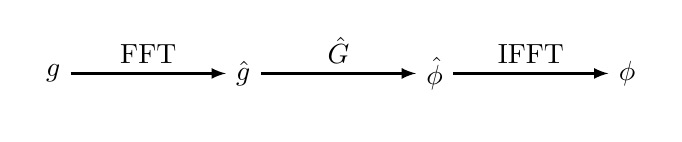
\begin{tikzpicture}[>=latex,thick]
	\matrix (m) [
		matrix of nodes,
		column sep=20mm,
		nodes={
			%line width=1pt,
			anchor=center,
			text centered,
			%minimum width=1cm,
			minimum height=8mm,
		},
%		txt/.style={text width=1.5cm,anchor=center},
	]
	{
		$g$ & $\hat g$ & $\hat \phi$ & $\phi$ \\%& $\E$\\
	};
	\foreach \i [evaluate={\j=int(\i+1)}] in {1,...,3}{
		\draw[->] (m-1-\i) -- (m-1-\j);
	}
	\draw[draw=none] (m-1-1) -- (m-1-2) node[midway,above] {FFT};
	\draw[draw=none] (m-1-2) -- (m-1-3) node[midway,above] {$\hat G$};
	\draw[draw=none] (m-1-3) -- (m-1-4) node[midway,above] {IFFT};
%	\draw[draw=none] (m-1-4) -- (m-1-5) node[midway,above]
%	{Eq.~\ref{eq:phi-to-E}};
\end{tikzpicture}
\end{center}%}}}
%
\begin{enumerate}
\item Compute the complex FFT $\hat g$ of $g$
\item Multiply each element of $\hat g$ by the corresponding complex coefficient 
$\hat G$, to obtain $\hat \phi$
\item Compute the inverse FFT of $\hat \phi$ to get $\phi$
\end{enumerate}
%
The complexity in the worst case is in $O(N_g \log_2 N_g)$ with the number of 
total points in the grid $N_g$.

\subsection{Electric field}
The electric field $\E$ can then be obtained by centered first order finite 
differences in each dimension
%
\begin{equation}%{{{
\begin{split}
\label{eq:phi-to-E}
\E_x(x,y) &= \frac{\phi(x-1,y) - \phi(x+1,y)}{2\,\Delta x} \\
\E_y(x,y) &= \frac{\phi(x,y-1) - \phi(x,y+1)}{2\,\Delta y}
\end{split}
\end{equation}%}}}
%

\section{Force interpolation}

The force acting on a particle $p$ can be decomposed in two main parts, the 
electric and magnetic force $\F=\F_E + \F_B$.

The electric force $\F_E$ is computed similarly as the charge deposition, but in 
the reverse order. The force $\F_E$ is interpolated from the electric field $\E$ 
of the neighbour grid points $\neigh{p}$, using the same interpolation function 
$W$.
\begin{equation}%{{{
\begin{split}
\F_E &= q \sum_{g \in \neigh{p}} W(\x_p - \x_g)\ \E(\x_g) \\
\end{split}
\end{equation}%}}}
Notice that a particle $p$ only needs the values of the electric field in the 
neighbourhood $\neigh{p}$.

The magnetic force $\F_B$ is constant in the simulator, as we only consider a 
fixed background magnetic field $\B_0$. For a particle $p$ with velocity $\v$  
can be written as
%
\begin{equation}%{{{
\F_B = q (\v \times \B_0)
\end{equation}%}}}


\section{Equations of motion}

In order to move the particles, the equations of motion need to be solved:
%
\begin{equation}
\frac{d\x}{dt}=\v
\end{equation}
\begin{equation}
m \frac{d\v}{dt} = \F
\end{equation}
%
The \textit{leap-frog} method is a common integration scheme with second-order 
accuracy and an error proportional to $\Delta t^2$. The name describes de 
behavior of the position and velocity, which are updated at interleaved time 
steps, similarly to the trajectory of a frog. The method is time reversible with 
an stability far superior of other higher-order integration methods, such as 
fourth order Runge-Kutta. A more in depth stability analysis can be found in 
Chapter 4 of Hockney and Eastwood book~\cite{hockney}.  The discretized 
equations can be written as
%
\begin{equation}
\frac{\x^{n+1} - \x^{n}}{\Delta \x} = \v^{n + 1/2}
\end{equation}
%
\begin{equation}
m\frac{\v^{n+1/2} - \v^{n-1/2}}{\Delta \x} = \F(x^n)
\end{equation}
%
Several methods are available, but we will focus on the Boris integrator.

\subsection{Boris integrator}

Consists of three steps:
%
\begin{enumerate}
\item Add half of the electric impulse
\item Rotate
\item Add the remaining half electric impulse
\end{enumerate}
%
The Boris integrator computes the velocity of a particle in a constant electric 
field $\E$ and a constant magnetic field $\B$. We have the velocity 
$\v_{t-\Delta t/2}$ of the particle at $t-\Delta t/2$ as we use the leapfrog 
integrator.
%
\begin{figure}[h]
\centering
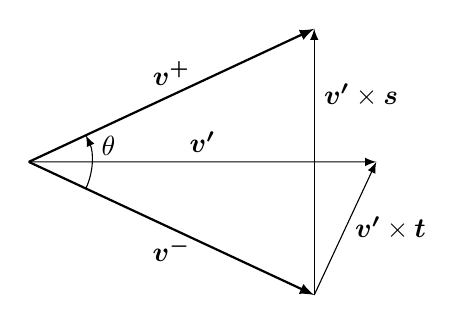
\begin{tikzpicture}[
	scale=2,
	>=latex]

	\def\centerarc[#1](#2)(#3:#4:#5)% Syntax: [draw options] (center) (initial angle:final angle:radius)
		{\draw[#1] ($(#2)+({#5*cos(#3)},{#5*sin(#3)})$) arc (#3:#4:#5); }

	\def\startangle{-25}
	\def\midangle{0}
	\def\endangle{25}
	\def\radius{2.0}
	\pgfmathsetmacro{\vlen}{\radius*tan(\startangle)}%

	\coordinate (O) at (0,0);
	\coordinate (S) at (\startangle:\radius);
	\coordinate (E) at (\endangle:\radius);

%	\centerarc[dashed](O)(\startangle:\endangle:\radius);
	\centerarc[->](O)(\startangle:\endangle:0.2*\radius);

	\draw (O)+(0.4,0.1) node [right] {$\theta$};

	\draw [thick,->] (O) -- (E) node [midway, above] {$\V{v^+}$};
	\draw [thick,->] (O) -- (S) node [midway, below] {$\V{v^-}$};

	\path (S) +(\startangle-90:\vlen) coordinate (V1E);
%	\path (E) +(\endangle-90:\vlen) coordinate (V3E);

%	%\draw [->] (E) -- (V3E);
	\draw [->] (S) -- (V1E) node [midway, right] {$\V{v'} \times \V t$};
%
	\draw [->] (O) -- (V1E) node [midway, above] {$\V{v'}$};
	\draw [->] (S) -- (E) node [near end, right] {$\V{v'} \times \V s$};

%	\draw [fill=white] (O) circle (0.02);

\end{tikzpicture}
\caption{Velocity space rotation from $\v-$ to $\v+$}
\end{figure}
%
\paragraph{Add half electric impulse} We define $\V{v^-}$ as the velocity after 
half a electric impulse:
$$\v^- = \v_{t-\dt/2} + \frac{q \E}{m} \frac{\dt}{2}$$

\paragraph{Rotate for the magnetic field} The rotation is done in two steps, 
first the half rotation is computed, with an angle of $\theta/2$:
$$\v' = \v^- + \v^- \times \V t $$

Then the rotation is completed by symmetry, using the $\V s$ vector
$$ \V s = \frac{2 \V t}{1 + \V t^2} $$
as
$$ \V{v^+} = \V{v^-} + \V{v}' \times \V{s} $$


\part{Copmutation\\ \small \textit{No more physics now}}

\chapter{Parallelization techniques}
\label{ch:techniques}

\section{Message Passing Interface}

From the need of standarize communications in a distributed computing
environment, the first draft was proposed in 1992 at the Workshop on Standards
for Message Passing in a Distributed Memory Environment, and has now become one
of the most used communication protocol in HPC. The Message Passing Interface
(MPI) provides a simple to use set of routines to allow processes distributed
among different nodes to comunicate efficiently.

\subsection{Concepts}


\paragraph{Communicator} A communicator refers to a group of processes, in which
each has assigned a unique identifier called the \textit{rank}.

\paragraph{Point-to-point communication} In order for a process to exchange
information with another process, the MPI standard defines what are called
point-to-point communication routines. The most common examples are
\texttt{MPI\_Send} to send data, and \texttt{MPI\_Recv} for the reception.
Both routines need the process rank of the process to stablish the connection.
Additionally a tag is used to label each message, which can be specified in the
reception to filter other messages.

\paragraph{Blocking communication} The standard defines various types of
communication methods for sending and receiving data. The so called blocking
routines are designed such that the call does not return until the communication
has been done. In the \texttt{MPI\_Send} case, the call returns when the sending
data can be safely modified, as has been sent or buffered. In the case of
\texttt{MPI\_Recv} the routine only returns when the data has been received.

\paragraph{Non-blocking communication} Similarly as with the blocking
communication, the routines \texttt{MPI\_Isend} and \texttt{MPI\_Irecv} don't
wait until the message is sent or received to return. They return inmediately,
and the communication status can be checked with \texttt{MPI\_Test} or the
process can wait until the communication request has finished with
\texttt{MPI\_Wait}.

\subsection{Implementations}


\section{OmpSs-2}

OmpSs-2 is the next generation of the OmpSs programming model, composed of a set
of directives and library routines. Mixes from OpenMP the annotation of source
code to parallelize some sections with the StarSs execution model, based on a
data-flow execution model.

\subsection{Concepts}

\paragraph{Task} In OmpSs-2 a task is a section of code that can be executed
independently by the runtime schedule. A task may have associated dependencies
which lets the scheduler determine in wich order is allowed to execute the
tasks. The notation used to describe a task is by the utilization of the
\texttt{\#pragma} directive, for example:
%
\begin{lstlisting}
#pragma oss task inout(a[0:N-1]) in(b[0:N-1])
for(i=0; i < N; i++)
	a[i] += b[i];
\end{lstlisting}
%

\paragraph{Parallel execution} Unless there is a unmet dependency, all tasks 
ready to run are executed in parallel, up to the number of CPU cores available 
to the runtime.

\paragraph{Task syncronization} It may be possible that at some point in the
execution all pending task are required to finish in order to continue. The
directive \texttt{taskwait} allows the programmer to specify that the runtime
must wait for completion of all previous created tasks.

\chapter{Simulator design}

[This chapter will be merged with the next one, is only here to keep the
numbering of the chapters, while I'm working on the comments]

\chapter{The simulator}
\label{ch:parallel-simulator}

\section{Decomposition}

To parallelize the simulation, the process must be decomposed in parts that can 
be executed in parallel and several decompositions are known.
%
One of the most common technique found in particle-in-cell codes, is the 
\textit{domain decomposition}---the physical space is divided into sections of 
similar size and the fields are assigned to different computing units. The main 
drawback of this technique is the risk of unbalanced load, as some regions of 
space may contain a large amount or even all the particles.

Another approach called \textit{particle decomposition} consists in the division 
of the particles into groups, where each processor maintains a copy of the 
fields of the whole space.  The problem of this method is the limitation of 
scalability, as the number of grid points used in the fields is limited by the 
memory of one computing element.

Additionally, the Fourier transform needed by the MFT solver is implemented 
using the FFTW library and the parallelization design provided by the library 
introduces a constraint in the distribution of the fields: they need to be 
broken into slices in the Y dimension, resulting in contiguous blocks of 
elements in X. Consequently, the domain decomposition is the chosen technique 
for the simulator.

\begin{figure}[ht]%{{{
\centering
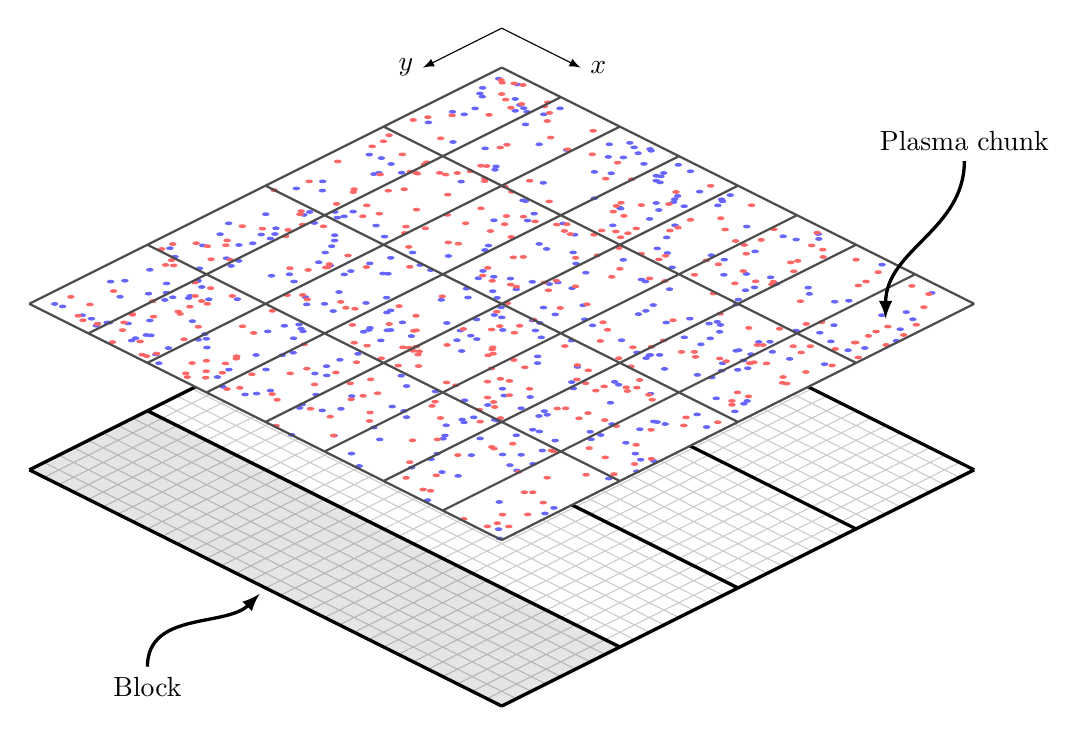
\begin{tikzpicture}
\begin{scope}[
		x=1cm,
		y=1cm,
		yshift=0,
		every node/.append style={
			yslant=0.5,xslant=-1},
		yslant=0.5,
		xslant=-1
	]
	% opacity to prevent graphical interference
	\draw[step=1.5/8, black!20!white, thin] (0,0) grid (6,6); %defining grids
	%\draw[step=1.5, black] (0,0) grid (6,6);
	\draw[xstep=1.5, ystep=6, black, very thick] (0,0) grid (6,6);
	%\draw[dashed, xstep=6, ystep=1.5, black] (0,0) grid (6,6);
	\fill[fill=black,fill opacity=0.1] (0,0) rectangle (1.5,6);
	\coordinate (a0) at (4.5, 0);
	\coordinate (a1) at (6, 0);
	\coordinate (a2) at (4.5, 1.5);
	\coordinate (a3) at (6, 1.5);

	\coordinate (b) at (0,3);

\end{scope}
\begin{scope}[
		x=1cm,
		y=1cm,
		yshift=60,
		every node/.append style={
			yslant=0.5,xslant=-1},
		yslant=0.5,
		xslant=-1
	]
	\coordinate (b0) at (4.5, 0);
	\coordinate (b1) at (6, 0);
	\coordinate (b2) at (4.5, 1.5);
	\coordinate (b3) at (6, 1.5);
	\coordinate (c) at (4.5+0.75, 0.75/2);
	%Idem as above, for the n-th grid:
%	\draw[dotted] (a0) -- (b0);
%	\draw[dotted] (a1) -- (b1);
%	\draw[dotted] (a2) -- (b2);
%	\draw[dotted] (a3) -- (b3);
%
%	\draw[dashed] (a2) -- (a3);

	\fill[fill=white,fill opacity=1.0] (0,0) rectangle (6,6);
	\begin{axis}[width=7.5cm,height=7.5cm,
						axis lines=none,
						%hide axis,
						xmin=-1, xmax=1,
						ymin=-1, ymax=1,
						inner frame sep=0,
				]
	\addplot [blue!60!white, only marks,
		mark=*, samples=400, mark size=0.75] (rand, rand);
	\addplot [red!60!white, only marks,
		mark=*, samples=400, mark size=0.75] (rand, rand);
	\end{axis}
	%\draw[step=1.5, black, thick] (0,0) grid (6,6);
	\draw[xstep=1.5, ystep=1.5/2, black!70!white, thick] (0,0) grid (6,6);
	%\draw[dashed,xstep=6, ystep=1.5, black, thick] (0,0) grid (6,6);


	\coordinate (O) at (6.5, 6.5);
\end{scope}

\draw[-latex,very thick] (c)+(1,2) node[above]{Plasma chunk}
				to[out=-90,in=90] (c);
\draw[-latex,very thick,shorten >=3pt] (b)+(-1.5,-1) node[below]{Block}
				to[out=90,in=180+45] (b);

\begin{scope}[
		y={(-1cm,0.5cm)},x={(1cm,0.5cm)}, z={(0cm,1cm)},
	]
%	\coordinate (O) at (-3, 3.5, 0);
%	\draw[-latex] (O) -- +(1, 0,  0) node [right] {$x$};
%	\draw[-latex] (O) -- +(0, -1, 0) node [right] {$y$};
%	\coordinate (O) at (-0.75, -0.75, 0);
	\draw[-latex] (O) -- +(-1, 0,  0) node [left] {$y$};
	\draw[-latex] (O) -- +(0, -1, 0) node [right] {$x$};
\end{scope}
\end{tikzpicture}
\caption{Domain decomposition: The plasma is divided into chunks in both 
directions and the fields into blocks in the Y dimension only}
\label{fig:domain-decomposition}
\end{figure}%}}}

Firstly, the space domain is distributed in blocks by splitting the physical 
space in the Y dimension, as shown in the figure~\ref{fig:domain-decomposition}, 
and each block is assigned to an MPI process. As the simulation evolves, 
communications are needed to exchange information between processes. The 
particles enclosed within a block also are assigned to the same process in order 
to speed up the interpolation process. Furthermore, a second level of 
decomposition splits the particles of a process into plasma chunks, which can be 
processed in parallel. In this case communications within the chunks of a 
process are not needed as we can use shared memory to exchange information.  
Notice that the number of chunks can vary to fit the number of CPUs.

We will refer to a block to denote the region of space assigned to a process and 
the grid points contained in that region. On the other hand a chunk has also a 
region of space assigned of a block, but always is associated with a group of 
particles.

\section{Data layout}

Each block contains the three fields needed for the simulation: the charge 
density $\rho$, the electric potential $\phi$ and the electric field $\E$, which 
can be decomposed in the two components $E_x$ and $E_y$. As a consequence, a 
total of four matrices are needed to store the three fields.

\begin{figure}[h]%{{{
\centering
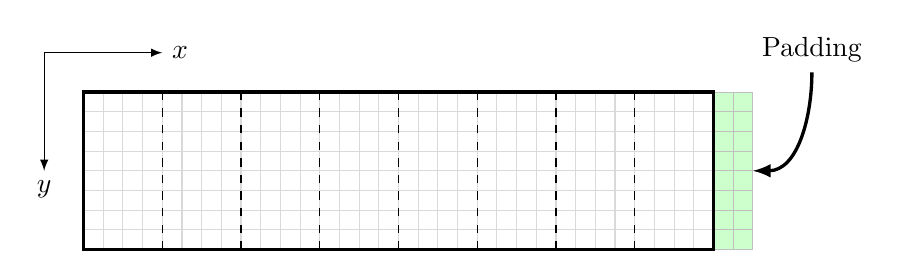
\begin{tikzpicture}[x=0.5cm,y=0.5cm]

\fill[green!20] (16,0) rectangle (17,4);
\draw[gray!30!white,step=0.5] (0,0) grid (16,4);
\draw[gray!50!white,step=0.5] (16,0) grid (17,4);
\draw[dashed,xstep=16/8,ystep=4] (0,0) grid (16,4);
\draw[very thick] (0,0) rectangle (16,4);

\coordinate (pad) at (17, 2);
\draw[-latex,very thick] (pad)+(1.5,+2.5) node[above] {Padding}
				to[out=-90,in=0] (pad);

\coordinate (O) at (-1, 5, 0);
\draw[-latex] (O) -- +(3, 0,  0) node [right] {$x$};
\draw[-latex] (O) -- +(0,  -3, 0) node [below] {$y$};
\end{tikzpicture}
\caption{A block divided in eight regions, each corresponding to a plasma chunk.  
Extra padding is added at the right for internal use in the FFTW library.}
\label{fig:block}
\end{figure}%}}}

A simplified representation of a block can be observed in the 
figure~\ref{fig:block}, where the X dimension of each field is contiguous in 
memory.  Notice the padding region in green, which is needed for the FFTW 
library to store intermediate values. The use of ghost elements is needed for 
communications and will be detailed in the chapter~\ref{ch:comm}. If we look at 
each cell $(x,y)$ in the block we find the four components $\rho(x,y)$, 
$\phi(x,y)$, $E_x(x,y)$ and $E_y(x,y)$.

\section{Simulation flow}

Before the main loop of the simulation begins, two previous iterations are 
required to prepare the simulation. The iteration counter is initially set to 
$-2$ to account for the extra steps.

\subsection{Allocation step}

After the creation of all MPI processes, the different structures to hold the 
data are allocated. Each process is assigned a block, with the corresponding 
fields and particles.

The fields are zeroed to begin the computation and the particles must be 
initialized following the user configuration. Each particle has an index which 
is used to let the user customize the particle attributes in case is required.  
Some initialization functions are provided, which place the particles following 
a random distribution or a specified pattern.

As the particles in a chunk are initialized, their position can set to any point 
in the physical space of the simulation, as no constraints are imposed for the 
initial placement. As a consequence, they need to be translated to the correct 
chunk before the simulation begins. We will refer to the initial movement of 
particles around the chunks as global communication, and is expected to last 
more than the typical communications once the simulation is running, as only 
local communications will be needed between neighbour chunks.

At soon as each particle is properly placed in the correct chunk, an initial 
computation of the charge density is done and the iteration counter is 
incremented.

\subsection{Rewind step}

The main loop begins with an special iteration that will only change the speed 
of the particles. The speed must be computed at half a time-step backwards in 
time, in order to use the leap-frog integrator as described in the 
section~\ref{sec:motion}. Once the iteration finishes, the main loop of can 
begin its normal execution with the iteration counter set to 0.

\subsection{Main loop}

The loop of the simulation performs four main steps:

\begin{itemize}
\item Accumulate charge density $\rho$ from the position of the particles.
\item Solve the field equation to get the electric field $\E$.
\item Interpolate the electric field $\E$ at particle positions.
\item Move the particles based on the computed force.
\end{itemize}

\section{Loop parallelization}

The four main steps of the simulation loop are parallelized following a common 
scheme: the block is partitioned in the same regions as the plasma chunks, which 
are processed in parallel.

\subsection{Charge accumulation}

%\begin{figure}[ht]%{{{
\begin{wrapfigure}{O}[2.7cm]{0.15\textwidth}
\centering
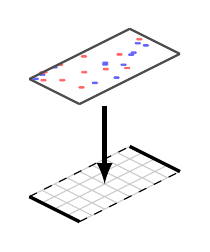
\begin{tikzpicture}[scale=0.85]
\begin{scope}[
		x=1cm,
		y=1cm,
		yshift=0,
		every node/.append style={
			yslant=0.5,xslant=-1},
		yslant=0.5,
		xslant=-1
	]
	\def\dx{0.0};
	% opacity to prevent graphical interference
	\draw[step=1.5/8, black!20!white, thin] (0,0-\dx) grid (6/4,6/8+\dx);
	%defining grids
	%\draw[step=1.5, black] (0,0) grid (6,6);
	\draw[xstep=1.5, ystep=0, black, very thick] (0,0-\dx) grid
		(6/4,6/8+\dx);
	\draw[dashed, xstep=6, ystep=1.5/2, black] (0,0) grid (6/4,6/8);

	\coordinate (b) at (1.5/2, 0.75/2);

\end{scope}
\begin{scope}[
		x=1cm,
		y=1cm,
		yshift=50,
		every node/.append style={
			yslant=0.5,xslant=-1},
		yslant=0.5,
		xslant=-1
	]
	\coordinate (c) at (1.5/2, 0.75/2);

	%\fill[fill=white,fill opacity=1.0] (0,0) rectangle (6,6);
	\begin{axis}[width=3cm,height=2.35cm,
						axis lines=none,
						%hide axis,
						xmin=-1, xmax=1,
						ymin=-1, ymax=1,
						inner frame sep=0,
				]
	\addplot [blue!60!white, only marks,
		mark=*, samples=12, mark size=0.75] (rand, rand);
	\addplot [red!60!white, only marks,
		mark=*, samples=12, mark size=0.75] (rand, rand);
	\end{axis}
	%\draw[step=1.5, black, thick] (0,0) grid (6,6);
	\draw[xstep=1.5, ystep=1.5/2, black!70!white, thick] (0,0) grid (6/4,6/8);
	%\draw[dashed,xstep=6, ystep=1.5, black, thick] (0,0) grid (6,6);


	\coordinate (O) at (1.5+0.5, 0.75+0.5);
\end{scope}

%\draw[-latex,very thick] (c)+(1,2) node[above]{Plasma chunk}
%				to[out=-90,in=90] (c);
%\draw[-latex,very thick,shorten >=3pt] (b)+(-1.5,-1) node[below]{Block}
%				to[out=90,in=180+45] (b);
\draw[-latex,ultra thick,shorten <=0.5cm]
	(c) to[out=-90,in=90] (b);
%	(c) to[out=-90,in=90]  node[midway,right]{Interpolation} (b);

\begin{scope}[
		y={(-1cm,0.5cm)},x={(1cm,0.5cm)}, z={(0cm,1cm)},
	]
%	\coordinate (O) at (-3, 3.5, 0);
%	\draw[-latex] (O) -- +(1, 0,  0) node [right] {$x$};
%	\draw[-latex] (O) -- +(0, -1, 0) node [right] {$y$};
%	\coordinate (O) at (-0.75, -0.75, 0);
%	\draw[-latex] (O) -- +(-1, 0,  0) node [left] {$y$};
%	\draw[-latex] (O) -- +(0, -1, 0) node [right] {$x$};
\end{scope}
\end{tikzpicture}
%\caption{Interpolation of the electric field $\E$ to the particles in a chunk.}
%\label{fig:interpolation-E}
\end{wrapfigure}
%\end{figure}%}}}
%
The interpolation process described in the equation~\ref{eq:charge-accumulation} 
is executed in parallel for all the particles of each chunk. The charge density 
field is being updated in parallel, which involves the four surrounding grid 
points of a particle, and it may happen that at the frontier of two chunks a 
concurrent access to the same element occurs.

To avoid a race condition with the next chunk, a dependency is added with the 
directive \texttt{commutative}, which allows the execution of the tasks in any 
order, but guarantees that a chunk can only be acessed by one task at a time. A 
detailed discussion on the directive can be found in the 
section~\ref{sec:exchange-x} with other alternatives to avoid a chain of 
dependencies in the case \texttt{inout} was used.

\begin{figure}[h]
\begin{lstlisting}[caption={Task to update $\rho$ field using the 
\texttt{commutative} directive}, captionpos=b]
for (i=0; i<plasma->nchunks; i++)
{
	c0 = &plasma->chunks[i];
	c1 = &plasma->chunks[(i + 1) % plasma->nchunks];
	#pragma oss task commutative(*c0, *c1) label(rho_update_0)
	rho_update(sim, i);
}
\end{lstlisting}
\end{figure}
% XXX Notice that we cannot have commutative in the next step or in the previous
% otherwise we can get ot of order execution in a chunk.

\subsection{Solve the fields}

Once the charge density is accumulated for each chunk, the electric potential 
can be computed by solving the Poisson equation (Eq.~\ref{eq:poisson}).  Using 
the MFT solver requires the computation of the Fourier transform of the charge 
density field, which has been purposely distributed among the Y dimension into 
blocks: The computation of the FFT can then be distributed into each process.

To parallelize the execution in each process, two mechanism are available in the 
FFTW library: pthreads and OpenMP. The multithreading design is based on the 
model of the \textit{parallel for}, where the total number of iterations are 
divided into parts that can be executed in parallel.
%
\begin{figure}[ht]%{{{
\begin{lstlisting}[
	%float,
	label={lst:openmp-for},
	caption={Parallel for with OpenMP used in the FFTW library.}]
#pragma omp parallel for private(d)
for (i = 0; i < nthr; ++i) {
	...
	proc(&d);
}
\end{lstlisting}
\end{figure}%}}}
%
In the listing~\ref{lst:openmp-for} the OpenMP parallelization method is shown, 
as used in the FFTW. With minor changes we can adapt the model to OmpSs-2, 
following the same approach. A task is created for each iteration and then we 
wait for the completion of all of them, ensuring all iterations of the loop have 
been executed, as can be seen in the listing~\ref{lst:ompss-for}. A comparative 
analysis of the different methods is provided in the chapter~\ref{ch:analysis}.
%
\begin{figure}[ht]%{{{
\begin{lstlisting}[
	%float,
	label={lst:ompss-for},
	caption={Parallel for with OmpSs-2 using tasks.}]
for (i = 0; i < nthr; ++i) {
	#pragma oss task private(d)
	{
		...
		proc(&d);
	}
}
#pragma oss taskwait
\end{lstlisting}
\end{figure}%}}}
%

Once we obtain the electric potential $\phi$ after the MFT algorithm, we can 
compute the electric field $\E$ in both directions $E_x$ and $E_y$. The 
operation can be fully parallelized in tasks by the division of the block in the 
same regions as the plasma chunks. It is not necessary that the same division is 
used, but has the advantage of simplify how the dependencies between plasma and 
fields are written.
%
\begin{figure}[ht]%{{{
\begin{lstlisting}[
label={lst:compute-E},
caption={Computation of E in parallel by chunks.}]
for(ic=0; ic<sim->plasma.nchunks; ic++)
{
	chunk = &sim->plasma.chunks[ic];
	#pragma oss task inout(*chunk) label(field_E_compute)
	field_E_compute(sim, chunk);
}
\end{lstlisting}
\end{figure}%}}}
%
The same division provided by the plasma chunks is used as a first approximation 
as shown in the listing~\ref{lst:compute-E}, but other number of regions are 
possible.

\subsection{Field interpolation}
%
%\begin{figure}[ht]%{{{
\begin{wrapfigure}{O}[2.5cm]{0.15\textwidth}
\centering
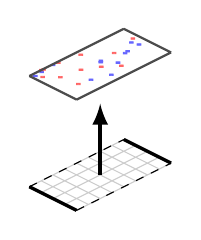
\begin{tikzpicture}[scale=0.8]
\begin{scope}[
		x=1cm,
		y=1cm,
		yshift=0,
		every node/.append style={
			yslant=0.5,xslant=-1},
		yslant=0.5,
		xslant=-1
	]
	\def\dx{0.0};
	% opacity to prevent graphical interference
	\draw[step=1.5/8, black!20!white, thin] (0,0-\dx) grid (6/4,6/8+\dx);
	%defining grids
	%\draw[step=1.5, black] (0,0) grid (6,6);
	\draw[xstep=1.5, ystep=0, black, very thick] (0,0-\dx) grid
		(6/4,6/8+\dx);
	\draw[dashed, xstep=6, ystep=1.5/2, black] (0,0) grid (6/4,6/8);

	\coordinate (b) at (1.5/2, 0.75/2);

\end{scope}
\begin{scope}[
		x=1cm,
		y=1cm,
		yshift=50,
		every node/.append style={
			yslant=0.5,xslant=-1},
		yslant=0.5,
		xslant=-1
	]
	\coordinate (c) at (1.5/2, 0.75/2);

	%\fill[fill=white,fill opacity=1.0] (0,0) rectangle (6,6);
	\begin{axis}[width=3cm,height=2.35cm,
						axis lines=none,
						%hide axis,
						xmin=-1, xmax=1,
						ymin=-1, ymax=1,
						inner frame sep=0,
				]
	\addplot [blue!60!white, only marks,
		mark=*, samples=12, mark size=0.75] (rand, rand);
	\addplot [red!60!white, only marks,
		mark=*, samples=12, mark size=0.75] (rand, rand);
	\end{axis}
	%\draw[step=1.5, black, thick] (0,0) grid (6,6);
	\draw[xstep=1.5, ystep=1.5/2, black!70!white, thick] (0,0) grid (6/4,6/8);
	%\draw[dashed,xstep=6, ystep=1.5, black, thick] (0,0) grid (6,6);


	\coordinate (O) at (1.5+0.5, 0.75+0.5);
\end{scope}

%\draw[-latex,very thick] (c)+(1,2) node[above]{Plasma chunk}
%				to[out=-90,in=90] (c);
%\draw[-latex,very thick,shorten >=3pt] (b)+(-1.5,-1) node[below]{Block}
%				to[out=90,in=180+45] (b);
\draw[-latex,ultra thick,shorten >=0.5cm]
	(b) to[out=90,in=-90] (c);
%	(b) to[out=90,in=-90]  node[midway,right]{Interpolation} (c);

\begin{scope}[
		y={(-1cm,0.5cm)},x={(1cm,0.5cm)}, z={(0cm,1cm)},
	]
%	\coordinate (O) at (-3, 3.5, 0);
%	\draw[-latex] (O) -- +(1, 0,  0) node [right] {$x$};
%	\draw[-latex] (O) -- +(0, -1, 0) node [right] {$y$};
%	\coordinate (O) at (-0.75, -0.75, 0);
%	\draw[-latex] (O) -- +(-1, 0,  0) node [left] {$y$};
%	\draw[-latex] (O) -- +(0, -1, 0) node [right] {$x$};
\end{scope}
\end{tikzpicture}
%\caption{Interpolation of the electric field $\E$ to the particles in a chunk.}
%\label{fig:interpolation-E}
\end{wrapfigure}
%\end{figure}%}}}
%
Once the electric field of a chunk is ready, the value is interpolated at the 
particle locations. The force will be obtained in the next step from the 
interpolated electric field in each particle.

Each chunk can be processed independently by one task, but a \texttt{inout} 
dependency must be added to ensure the order of execution of a chunk is done 
after the electric field is computed, as observed in the 
listing~\ref{lst:interpolate-E}.
%
\begin{figure}[ht]%{{{
\begin{lstlisting}[
label={lst:interpolate-E},
caption={Interpolation of the electric field $\E$ at particle position.}]
for(i=0; i<sim->plasma.nchunks; i++)
{
	chunk = &sim->plasma.chunks[i];
	#pragma oss task inout(*chunk) label(chunk_E)
	{
		for(is=0; is<chunk->nspecies; is++)
		{
			particle_set_E(sim, chunk, is);
		}
	}
}
\end{lstlisting}
\end{figure}%}}}
%
\subsection{Particle mover}

The force acting on each particle is obtained as described in the 
equation~\ref{eq:force}, as the combination of the electric and magnetic forces.  
The electric term is computed from the interpolated electric field at the 
particle locations and each chunk can begin the process as soon as the 
interpolation process has finished.

A task is created for each chunk, and the particles are moved accordingly to the 
obtained force. The Boris integrator described in the section~\ref{sec:boris} is 
used to accurately position the particles. An \texttt{inout} dependency is added 
to each chunk to guarantee the order of execution: after the electric field is 
interpolated in the particles, as shown in the listing~\ref{lst:particle-mover}.
%
\begin{figure}[ht]%{{{
\begin{lstlisting}[
label={lst:particle-mover},
caption={Movement of particles based on the interpolated field $\E$.}]
for(i=0; i<sim->plasma.nchunks; i++)
{
	chunk = &sim->plasma.chunks[i];
	#pragma oss task inout(*chunk) label(chunk_x_update)
	{
		for(is=0; is<chunk->nspecies; is++)
		{
			particle_x_update(sim, chunk, is);
		}
	}
}
\end{lstlisting}
\end{figure}%}}}

\chapter{Analysis}


%\section{Analyze time distribution}

In order to reduce the amount of CPU time involved in each step of the 
simulation, the best strategy is to reduce the time spent in the most time 
consuming part.

The CPU time involved in each part of the simulation may depend on various 
factors, such as the number of grid points, the number of particles or the 
boundary conditions. As an example, consider a simulation with a large number of 
grid points, with few particles---the computation of the electric field 
(\texttt{field\_E}) will dominate the simulation time, as shown in the figure 
\ref{fig:cm-big-grid}. In a case of a large number of particles and a smaller 
grid, the particle interpolation (\texttt{particle\_E}) dominates the whole 
execution as seen in the figure \ref{fig:cm-lots-particles}.
%
\begin{figure}[h]
	\centering
	\subfloat[1024 particles, 512x512 grid points]{
		\includegraphics[width=0.95\linewidth]{callmap-grid512x512-n1024.png}
		\label{fig:cm-big-grid}
	}
	\\
	\subfloat[10240 particles, 64x64 grid points]{
		\includegraphics[width=0.95\linewidth]{callmap-grid64x64-n10240.png}
		\label{fig:cm-lots-particles}
	}
	\caption{Comparison of the time spent in each function at two different 
	simulations.}
\end{figure}
%
In order to optimize the general use case, different inputs will be tested and 
the main simulation steps will be characterized. Furthermore, different 
algorithms or methods may be used to improve the speed. As an example, the LU 
algorithm is compared with the spectral method MFT.

\section{Analysis with varying inputs}

\chapter{Caveats and limitations}

Here is a list of things that are not implemented in the simulator, but may be 
added in a future work.

\begin{itemize}
\item More than 2 dimensions
\item Fully electromagnetic simulation
\item Relativistic particle movement
\item Heterogeneous architecture (GPU+CPU...)
\item Energy conserving codes
\item Visualization of big simulations (paraview)
\end{itemize}
%
Caveats that need to be fixed
%
\begin{itemize}
\item Allow to specify plasma frequency
\item Validation with other simulation codes
\end{itemize}


%
%\chapter{Results}
%
%\chapter{Conclusions}

\bibliographystyle{siam}
\bibliography{bib}

\end{document}
